\documentclass[a4paper]{article}
\usepackage[affil-it]{authblk}
\usepackage{etoolbox}
\usepackage{setspace}
\usepackage{amssymb}
\usepackage{amsthm}
\usepackage{mathtools}
\usepackage{url}
\usepackage{pdfpages}
\usepackage[margin=1.4in]{geometry}

\DeclarePairedDelimiter{\ceil}{\lceil}{\rceil}

\AtBeginEnvironment{quote}{\singlespacing\small}

\theoremstyle{definition}
\newtheorem{definition}{Definition}[section]
\newtheorem{claim}[definition]{Claim}

\title{Seat apportionment in the European Parliament and Brexit}
\author{Karel Jílek}
\affil{ETH Zürich}

\begin{document}
\maketitle
\clearpage

\section{Introduction}
On 23rd June 2016, citizens of the United Kingdom decided in the European Union membership referendum to leave the EU (so-called Brexit).\textsuperscript{\cite{brexit}} Since then, there have been discussions about how to leave the EU, but as of December 2019, the UK is still a member. On 12th December 2019, Boris Johnson, a politician who is strongly for Brexit, won general election in the UK, resulting in 365 seats won out of the total of 650 seats\textsuperscript{\cite{election}}, and became the prime minister. With such a majority in the House of Commons, things might finally start to move, and the UK could leave the EU as of 31st January, 2020.\textsuperscript{\cite{brexit}}

One of the aspects of leaving the EU is that the seats of the leaving country in several EU institutions need to be handled. One of those institutions is the European Parliament, often abbreviated as EP.

It is already decided how the seats belonging to the UK will be redistributed among the remaining members of the EU. Once the UK actually leaves, out of the current 73 British seats, 27 are planned to be reassigned, while the remaining 46 will be empty, effectively shrinking the size of the Parliament from 751 seats down to 705.\textsuperscript{\cite{shrink}} There are already some questions: Why not just reassign all the seats? How come that the shrink has the size of 46? But before the answers, one needs to understand how the  apportionment in the EP actually works.

This paper elaborates on the seat apportionment in the European Parliament and tries to answer those questions.

\section{Seat Apportionment in the EP}

The seat apportionment method used for the European Parliament is defined in the Treaty on European Union, Art. 14, par. 2:\textsuperscript{\cite{eutreaty}}

\begin{quote}
	\textit{The European Parliament shall be composed of representatives of the Union's citizens. They shall not exceed seven hundred and fifty in number, plus the President. Representation of citizens shall be degressively proportional, with a minimum threshold of six members per Member State. No Member State shall be allocated more than ninety-six seats.}
\end{quote}

To be more expressive, building a mathematical model should help. Let $S$ be the tuple of EU member states.

\begin{definition}
	 \textit{Apportionment method}\textsuperscript{\cite[p.~55]{slides}} $$A: \{S\} \times \mathbb{N}^{|S|} \times \mathbb{N} \rightarrow \mathbb{N}^{|S|}$$ takes the tuple of member states, their populations and the parliament size and yields the number of seats allocated for each member state, let it be $(a_1, a_2, ..., a_{|S|})$. Then,  $\sum (a_1, a_2, ..., a_{|S|})$ is equal to the parliament size (the whole parliament is distributed).
\end{definition}
Let $P \in \mathbb{N}$ be the size of the European Parliament, $A_{EP}$ be the apportionment method used to calculate the seat allocation in the EP, and $p \in \mathbb{N}^{|S|}$ the populations used in that calculation. Then, from the EU Treaty paragraph shown above, the following could be derived (degressive proportionality will be discussed in a moment):
\begin{align}
P &\le 751 \label{rule1} \\
\min A_{EP}(S, p, P) &\ge 6 \label{rule2} \\
\max A_{EP}(S, p, P) &\le 96 \label{rule3}
\end{align}. 

The Treaty of Lisbon from December 2009\textsuperscript{\cite{lisbontreaty}} grants the right to decide the actual apportionment to the European Council.\textsuperscript{\cite{wikilisbontreaty}}

These rules do not just look ambiguous -- they really are. That is probably one of many reasons why Cambridge Compromise took place in 2011. It refines the definition of degressive proportionality so that it can be used for the need of seat apportionment in the EP, and also, it suggests an apportionment method.\textsuperscript{\cite{cambridge}} As per the Compromise, to be \textit{degressively proportional} means the following: \textsuperscript{\cite[p.~11]{cambridge}}

\begin{quote}
	\textit{The principle of degressive proportionality means that the ratio between the population and the number of seats of each	Member State \textbf{before rounding to whole numbers} must vary in relation to their respective populations in such a way that each Member from a more populous Member State represents more citizens than each Member from a less populous Member State and conversely, but also that no less populous Member State has	more seats than a more populous Member State.}
\end{quote}

The bold part is bold also in the original text and it is really important. For more details, see \cite[p.~10]{cambridge}.

Translated into the language of mathematics:

\begin{definition}
	Let $A$ be an apportionment method. \textit{Apportionment method without rounding} $$A^*: \{S\} \times \mathbb{N}^{|S|} \times \mathbb{N} \rightarrow \mathbb{R}^{|S|}$$ takes the same parameters as $A$ and yields an apportionment without rounding. If rounding was applied in $A^*$, then  $A^* = A$.
\end{definition}

Let $A^*_{EP}$ be the apportionment method used to calculate the seat allocation in the EP, but without rounding. Then (note that $S_i$ stands for i-th item of tuple $S$):

\begin{align}
\forall i,j \in  1, ... ,|S|: p_i \ge p_j &\implies A_{EP}^*(S, p, P)_i \ge A_{EP}^*(S, p, P)_j \label{rule4} \\ 
\forall i,j \in  1, ... ,|S|: p_i \ge p_j &\implies \frac{p_i}{A_{EP}^*(S, p, P)_i} \ge \frac{p_j}{A_{EP}^*(S, p, P)_j} \label{rule5}
\end{align}

The apportionment method suggested by Cambridge Compromise is \textit{base+prop} method: each member is apportioned a \textit{base} number of seats, and then the remaining seats are distributed \text{proportionally} by the population of the members. More specifically:\textsuperscript{\cite[p.~12]{cambridge}}
\begin{itemize}
	\item assign to each member a \textit{base} number of seats, denoted as $b$,
	\item take a divisor $d$ and assign to each member $i$ additional $p_i/d$ seats, where $p_i$ is the population of member $i$,
	\item perform a rounding so that each member has an integral number of seats; if this number exceeds the maximum, use the maximum instead,
	\item if the sum of all assigned seats is not equal to the Parliament size, adjust $d$.
\end{itemize}

Cambridge Compromise suggests values $b=5$ and rounding upwards\textsuperscript{\cite[p.~12]{cambridge}}, which guarantees that each member gets at least 6 seats.\footnote{Provided it has a non-zero population.}

In 2013, the European Council released a decision which established the composition of the European Parliament, being effective from  the parliamentary term 2014 -- 2019 until Brexit actually happens.\textsuperscript{\cite{ec2013}} It implements rules (\ref{rule4}) and (\ref{rule5}) and strengthens rules (\ref{rule2}) and (\ref{rule3}) by saying that $\min A_{EP}(S, p, P) = 6$ and $\max A_{EP}(S, p, P) = 96$ to ``\textit{reflect  as  closely  as  possible  the  sizes  of  the  respective  populations  of  Member  States}"\textsuperscript{\cite[Art.~1]{ec2013}}. From the proposed apportionment\textsuperscript{\cite[Art.~3]{ec2013}}, by summing up all the seats, it reveals that $P = 751$, thus strengthening also rule (\ref{rule1}). The Decision also mentions that the population data shall be taken from Eurostat\textsuperscript{\cite[Art.~2]{ec2013}}. Therefore, the newest population data available at the time of releasing the Decision is as of 1st January 2013\textsuperscript{\cite{eurostat}}.

However, the thing which is not followed in the Decision is the proposed apportionment method. Thus, the following can be said:

\begin{claim}
	$A_{EP}$, as defined by the Treaty on European Union\textsuperscript{\cite{eutreaty}} and the Decision of the European Council\textsuperscript{\cite{ec2013}} (that is, by rules from (\ref{rule1}) to (\ref{rule5})), is ambiguous.
\end{claim}

\begin{proof}
	Let $A_{B+P}$ be base+prop apportionment method with base 5 and upwards rounding. We show that $A_{B+P}$ also obeys the rules from (\ref{rule1}) to (\ref{rule5}) and $A_{B+P} \ne A_{EP}$. Compare those two apportionments in a table:
	\begin{figure}[th!]
		\begin{center}
			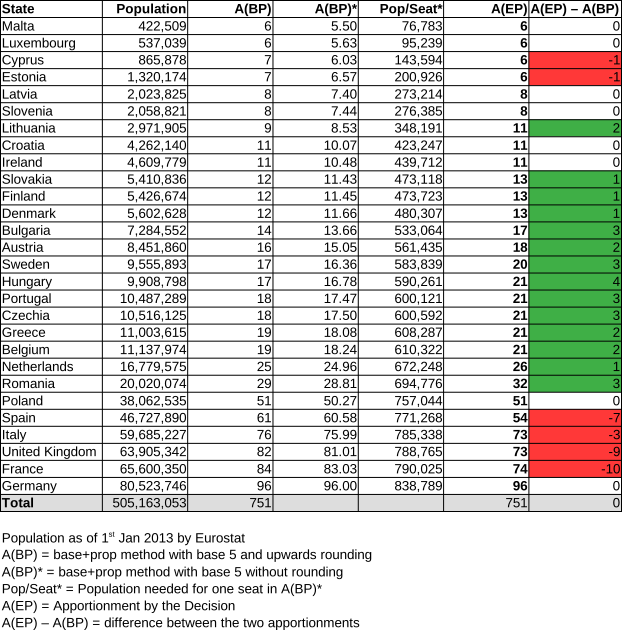
\includegraphics[scale=0.47]{g5202.png}
			\caption{Comparison of $A_{B+P}$ and $A_{EP}$. (Source: own calculation)}
			\label{fig:fig1}
		\end{center}
	\end{figure}

	$A_{B+P}$ clearly obeys rules (\ref{rule1}), (\ref{rule2}) and (\ref{rule3}): Malta being the least populous country gets 6 seats, Germany being the most gets 96 seats, and all 751 seats are distributed. Rule (\ref{rule4}) is also obeyed, as the population and the $A_{B+P}^*$ columns strictly increase and so does the \textit{Pop/Seat\textsuperscript{*}} column, which is what rule (\ref{rule5}) says. So $A_{B+P}$ follows all the requirements of $A_{EP}$, but clearly $A_{B+P} \ne A_{EP}$.
\end{proof}

While for example the law of Czech Republic in conjunction with Czech Statistical Office precisely define the method for apportionment in the Czech parliament\textsuperscript{\cite{csu}} (d'Hondt method\textsuperscript{\cite{dhondt}}), the European one seems not to be the case.\footnote{On 24 Dec 2019, I personally sent a query using the official contact form to ask the details about $A_{EP}$. No answer so far.}

Figure \ref{fig:fig1} shows that $A_{EP}$ tends to assign more seats to mid-size states while snatching seats from big states. The table below shows comparison of $A_{EP}$ with other used apportionment methods:

\begin{figure}[th!]
	\begin{center}
		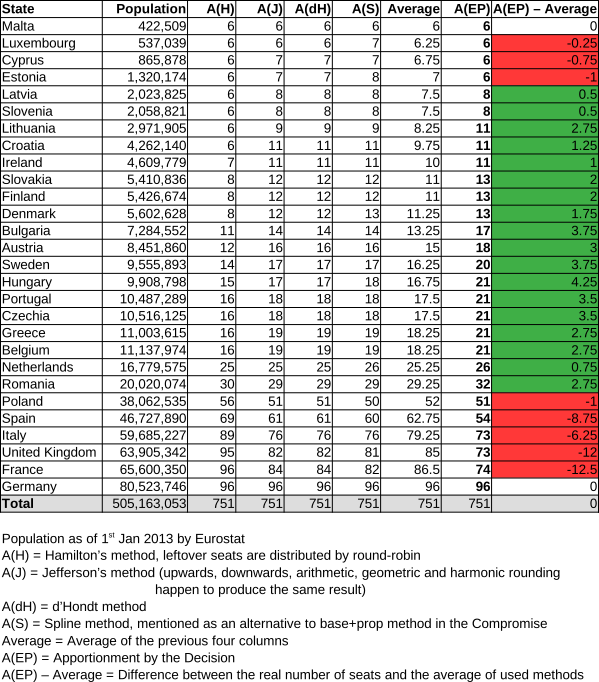
\includegraphics[scale=0.47]{g7093.png}
		\caption{Comparison of apportionment methods. (Source: own calculation; for more details, check the implementation at \cite{github}.)}
		\label{fig:fig2}
	\end{center}
\end{figure}
\pagebreak
It reveals that all of the conventional methods seem to prefer more populous member states. Maybe that is one of the reasons a new apportionment method was invented. Unfortunately, its details are not published, and it does not quite resemble any of the other methods.

\section{Redistribution of the British seats}

Basically, there are three options what to do with British seats: redistribute them, leave them empty, or a combination of both. The last option is the one which the European Council opted for: taking place -- 27 will be reassigned and 46 will remain empty\textsuperscript{\cite{ec2018}}. Again, there are no details of the apportionment method. The table in Figure \ref{fig:fig3} compares the new apportionment with other apportionment methods, using the newest population data by Eurostat at the time of releasing the Decision: that is 2018. Let $A_{BR}$ be the apportionment method used by the European Council for Brexit purposes.

\begin{figure}[th!]
	\begin{center}
		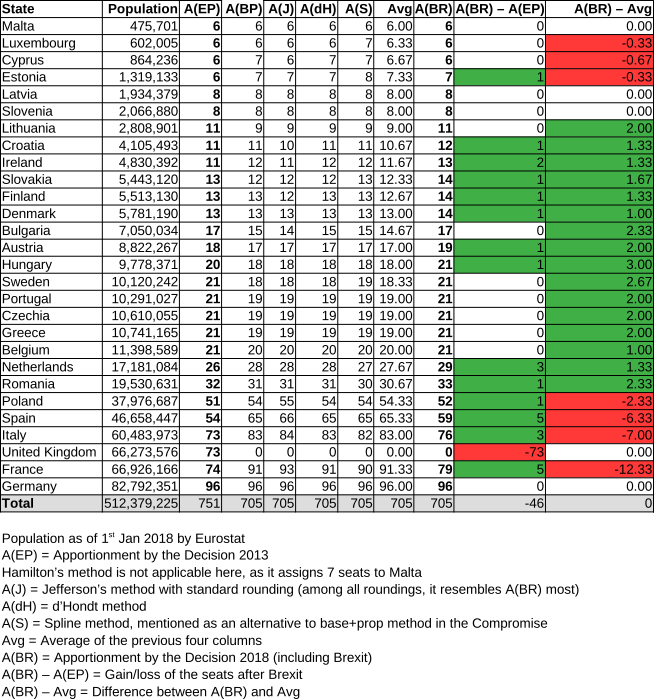
\includegraphics[scale=0.47]{g3522.png}
		\caption{Comparison of apportionment methods after Brexit. (Source: own calculation; for more details, check the implementation at \cite{github}.)}
		\label{fig:fig3}
	\end{center}
\end{figure}

$A_{BR}$ makes sure nobody loses their seats. Most of the seats are reassigned to the biggest states, which are, though, still quite underrepresented, compared to other apportionment methods. It could be said that they benefit the most, but at the price of still having not as many seats as they could have. Thus, the goal of the cut was probably not to hurt or let anyone benefit.

There is a much more likely scenario: currently, the Parliament is full, and thus nobody can join the European Union at the moment, as they would not get their at least 6 EP seats. According to Eurostat, the population of the EU on 1st January 2019 is 513 481 690, therefore, one seat out of 751 represents roughly 680 000 citizens. By freeing 46 seats, there is suddenly room for one or more states with the total population up to about 31 000 000 citizens to immediately join the EU -- without the cut, they would need to wait for the next parliamentary term. That is not enough for Ukraine, but almost all states at the Balkans could potentially fit.

\section{Conclusion}

While looking for the reasoning for the proposed redistribution of the British seats in the European Parliament, a much more serious problem arose: the apportionment method used in the EP is ambiguous and seem to produce quite different results from other, more common apportionment methods -- it reveals to be disadvantageous to more populous states. However, that is pretty much all we know. It would be definitely worth defining it properly!

The cut of size 46 allows to compensate the underrepresentation of big members a little bit and is decent to fit any single country in Europe and not (yet) in the EU except Ukraine and Russia immediately. Time will tell whether the cut was really needed.

\begin{thebibliography}{9}
	
	\bibitem{brexit}
	Wikipedia contributors. \textit{Brexit}. \url{https://en.wikipedia.org/w/index.php?title=Brexit&oldid=935613116}. 13 Jan 2020. [Online; cit. 30 Jan 2020]
	
	\bibitem{election}
    Elise Uberoi, Carl Baker, Richard Cracknell. \textit{General Election 2019: full results and analysis}. \url{https://researchbriefings.parliament.uk/ResearchBriefing/Summary/CBP-8749}. 19 Dec 2019. [Online; cit. 30 Jan 2020]
    
    \bibitem{shrink}
    EU Press. \textit{General Election 2019: full results and analysis}. \url{https://www.europarl.europa.eu/news/en/headlines/eu-affairs/20180126STO94114/eu-elections-how-many-meps-will-each-country-get-in-2019}. 7 Feb 2018. [Online; cit. 30 Jan 2020]
    
    \bibitem{eutreaty}
    Official Journal of the European Union. \textit{Consolidated Version of the Treaty on European Union}. \url{https://eur-lex.europa.eu/resource.html?uri=cellar:2bf140bf-a3f8-4ab2-b506-fd71826e6da6.0023.02/DOC_1&format=PDF}. 26 Oct 2012. [Online; cit. 30 Jan 2020]
    
    \bibitem{slides}
    Philip Grech. \textit{Mathematics in Politics and Law}. \url{https://moodle-app2.let.ethz.ch/pluginfile.php/763650/mod_resource/content/16/MATHEMATICS%20IN%20POLITICS%20AND%20LAW.pdf}. 2019. [Online; cit. 30 Jan 2020]
    	
    \bibitem{lisbontreaty}
    Eeva Pavy. \textit{Fact Sheet on the European Union: The Treaty of Lisbon}. \url{http://www.europarl.europa.eu/factsheets/en/sheet/5/the-treaty-of-lisbon}. Nov 2019. [Online; cit. 30 Jan 2020]
    
    \bibitem{wikilisbontreaty}
    Wikipedia contributors. \textit{Treaty of Lisbon}. \url{https://en.wikipedia.org/w/index.php?title=Treaty_of_Lisbon&oldid=937179628}. 23 Jan 2020. [Online; cit. 30 Jan 2020]
    
    \bibitem{cambridge}
    Geoffrey Grimmet and collaborators. \textit{The allocation between the EU Member States of the seats in the European Parliament}. \url{https://www.europarl.europa.eu/RegData/etudes/note/join/2011/432760/IPOL-AFCO_NT(2011)432760_EN.pdf}. 29 Jan 2011. [Online; cit. 30 Jan 2020]
    
    \bibitem{ec2013}
    European Council. \textit{EUROPEAN COUNCIL DECISION establishing the composition of the European Parliament}. \url{https://eur-lex.europa.eu/legal-content/EN/TXT/PDF/?uri=CELEX:32013D0312&from=EN}. 28 Jun 2013. [Online; cit. 30 Jan 2020]
    
    \bibitem{eurostat}
    Eurostat. \textit{Population on 1 January}. \url{https://ec.europa.eu/eurostat/databrowser/view/tps00001/default/table?lang=en}. 6 Nov 2019. [Online; cit. 30 Jan 2020]
    
    \bibitem{csu}
    Pavel Kuklík and Josef Baxa. \textit{Metody pro přepočet hlasů na mandáty}. \url{https://www.czso.cz/csu/czso/metody_pro_prepocet_hlasu_na_mandaty}. 3 Oct 2012. [Online; Czech; cit. 30 Jan 2020]
    
    \bibitem{dhondt}
    Wikipedia contributors. \textit{D'Hondt method}. \url{https://en.wikipedia.org/w/index.php?title=D%27Hondt_method&oldid=933523280}. 23 Jan 2020. [Online; cit. 30 Jan 2020]
    	
   	\bibitem{github}
   	Karel Jílek. \textit{ep-apportionment}. \url{https://github.com/karlosss/ep-apportionment/tree/e387d085a49755da8f14e14ff4b734b791c6656d}. 29 Jan 2020. [Online; GitHub repository; cit. 30 Jan 2020]
   	
   	\bibitem{ec2018}
   	European Council. \textit{EUROPEAN COUNCIL DECISION establishing the composition of the European Parliament}. \url{https://eur-lex.europa.eu/legal-content/EN/TXT/PDF/?uri=CELEX:32018D0937&from=EN}. 19 Jun 2018. [Online; cit. 30 Jan 2020]

\end{thebibliography}



\end{document}